\section{Outras Vertentes}

\subsection{Henry Briggs}
\begin{wrapfigure}{l}{0.3\textwidth}
    \setlength{\intextsep}{0pt}
    \vspace{-1.5em} 
    \centering
    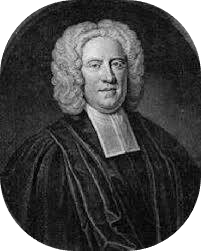
\includegraphics[width=\linewidth]{img/briggs.png} 
\end{wrapfigure}

Em 1616, impulsionado pela repercussão dos logaritmos, o matemático inglês Henry Briggs (1561 - 1630), professor de geometria no Gresham College, em Londres, ficou fascinado com a criação de Napier. Briggs visitou Napier em Edimburgo e sugeriu uma alteração na base do logaritmo. Com o intuito de tornar os cálculos mais intuitivos, ele propôs que o logaritmo fosse calculado na base decimal.

Napier concordou com a ideia; entretanto, faleceu logo em seguida, em 1617. Dessa forma, o encargo de adaptar as tabelas de logaritmos para a base decimal ficou a cargo de Briggs.

Em 1617, Briggs publicou os logaritmos dos primeiros 1.000 números. Já em 1624, lançou o livro \textit{Arithmetica Logarithmica}, uma obra contendo os logaritmos dos primeiros 30.000 números naturais, com 14 casas de precisão.

\begin{figure}[H]
    \centering
    
\includegraphics[height=9cm]{img/capa.png}
    \caption{Capa do Arithmetica Logarithmica}
\end{figure}

\begin{figure}[H]
    \centering
    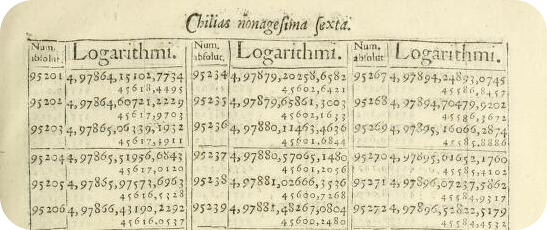
\includegraphics[height=4.5cm]{img/tabela1.png}
    \caption{Tabela desenvolvida por Briggs}
\end{figure}

\subsection{Jost Burgi}

\begin{wrapfigure}{l}{0.3\textwidth}
    \setlength{\intextsep}{0pt}
    \vspace{-1.5em} 
    \centering
    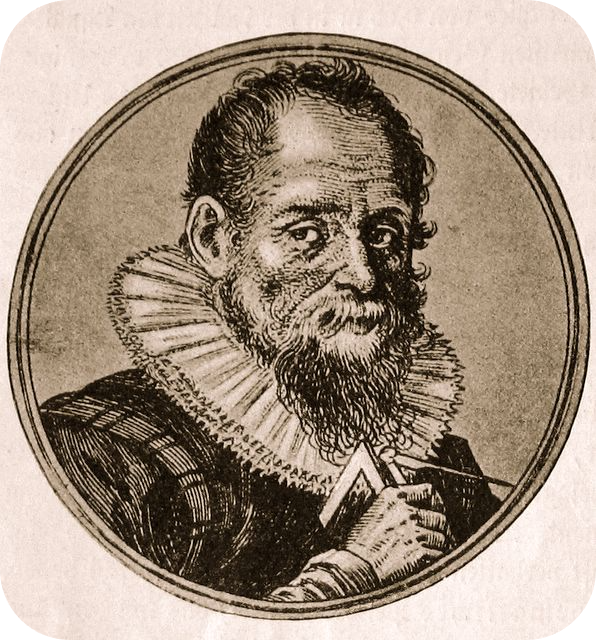
\includegraphics[width=\linewidth]{img/burgi.png} 
\end{wrapfigure} 

Por volta de 1600, o relojoeiro e matemático suíço Jost Bürgi (1552-1632) construiu uma tabela de progressões (um conceito análogo aos antilogaritmos) que precedeu os trabalhos de Napier, utilizando um método distinto. 

Ao desenvolver sua tabela, Burgi percebeu que utilizar bases simples, como por exemplo 2, fazia com que as potências crescessem muito rapidamente e, portanto, tornando impraticável seu uso para interpolação de valores. Como método de contornar tal problemática, Burgi adotou uma razão muito próxima de 1, em específico $1.0001$ como base para sua progressão geométrica.

Um dos aspectos mais distintos do sistema de Bürgi foi o uso de cores para enfatizar a relação dual entre a progressão aritmética (os logaritmos) e a progressão geométrica (os antilogaritmos).

Ao contrário de Napier, que desenvolveu uma terminologia técnica, Bürgi criou uma distinção visual imediata ao utilizar tinta preta e vermelha, tanto no texto explicativo quanto nas próprias tabelas:

\begin{itemize}
    \item \textbf{Números Vermelhos (Logaritmos):} Impressos em vermelho, representavam os argumentos da tabulação. Estes números seguiam uma progressão aritmética.
    
    \item \textbf{Números Pretos (Antilogaritmos):} Impressos em preto, representavam as entradas tabulares, ou os "números ordinários". Estes números seguiam a progressão geométrica de base $1.0001$.
\end{itemize}

\begin{figure}[H]
    \centering
    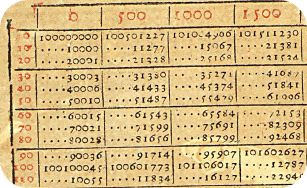
\includegraphics[height=5.5cm]{img/tabelaburgi.png}
    \caption{Tabela desenvolvida por Burgi}
\end{figure}

Apesar de a tabela de Bürgi ter, na prática, o mesmo propósito da de Napier — transformar multiplicações complexas em adições simples — e de ter sido criada anteriormente, ela não conseguiu estabelecer uma base teórica suficientemente clara para definir o conceito abstrato de função logarítmica.

Por essa razão histórica, e pela fundamentação conceitual mais robusta de seu trabalho publicado em 1614, John Napier é predominantemente reconhecido como o inventor dos logaritmos.